\begin{figure}
  \centering
    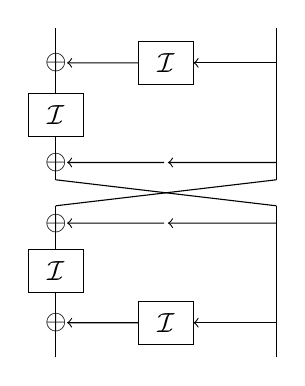
\begin{tikzpicture}[xscale=0.7, yscale=0.55]
      % TOP PART
      % -- cube
      \draw (-0.5, +2.5) rectangle node[pos=0.5]{$\mathcal{I}$} (+0.5, +3.5);
      % -- cube inverse
      \draw (-1.5, +1.3) rectangle node[pos=0.5]{$\mathcal{I}$} (-2.5, +2.3);
      % -- alpha multiplication
      \draw (+0.0, +0.7) node[inner sep=0](mult0){$\fmult$} ;
      \draw (+0.0, +1.2) node[inner sep=0]{$\WW$} ;
      % -- XORs
      \draw (-2.0, +3.0) node[inner sep=0](xor0){$\oplus$} ;
      \draw (-2.0, +0.7) node[inner sep=0](xor1){$\oplus$} ;
      % -- wires
      \draw (+2.0, +3.8) -- (+2.0, +0.3);
      \draw (-2.0, +3.8) -- (-2.0, +2.3);
      \draw[->] (+2.0, +3.0) -- (+0.5, +3.0);
      \draw[->] (-0.5, +3.0) -- (xor0);
      \draw[->] (+2.0, +0.7) -- (mult0);
      \draw[->] (mult0) -- (xor1);
      \draw (-2.0, +1.3) -- (-2.0, +0.3);
      % MIDDLE WIRING
      \draw (+2.0, +0.3) -- (-2.0, -0.3);
      \draw (-2.0, +0.3) -- (+2.0, -0.3);
      % BOTTOM PART
      % -- cube (xored)
      \draw (-0.5, -2.5) rectangle node[pos=0.5]{$\mathcal{I}$} (+0.5, -3.5);
      % -- cube
      \draw (-1.5, -1.3) rectangle node[pos=0.5]{$\mathcal{I}$} (-2.5, -2.3);
      % -- alpha multiplication
      \draw (+0.0, -0.7) node[inner sep=0](mult1){$\fmult$} ;
      \draw (+0.0, -1.2) node[inner sep=0]{$\WW$} ;
      % -- XORs
      \draw (-2.0, -3.0) node[inner sep=0](xor2){$\oplus$} ;
      \draw (-2.0, -0.7) node[inner sep=0](xor3){$\oplus$} ;
      % -- wires
      \draw (+2.0, -3.8) -- (+2.0, -0.3);
      \draw (-2.0, -3.8) -- (-2.0, -2.3);
      \draw[->] (+2.0, -3.0) -- (+0.5, -3.0);
      \draw[->] (-0.5, -3.0) -- (xor2);
      \draw[->] (+2.0, -0.7) -- (mult1);
      \draw[->] (mult1) -- (xor3);
      \draw (-2.0, -1.3) -- (-2.0, -0.3);
    \end{tikzpicture}  
    \FigDef{final-decomposition}{The APN involution $S_{\inv}$.}
\end{figure}

